\chapter{Results}
What are the measurement/model results

\section{Voltage measurements}

\Cref{fig:m_x1-x2} shows the signal X1 into the pulse shaper and the resulting signal X2 on the output of the pulse shaper. The interupter and power amplifier is not connected.

\begin{figure}[H]
    \centering
    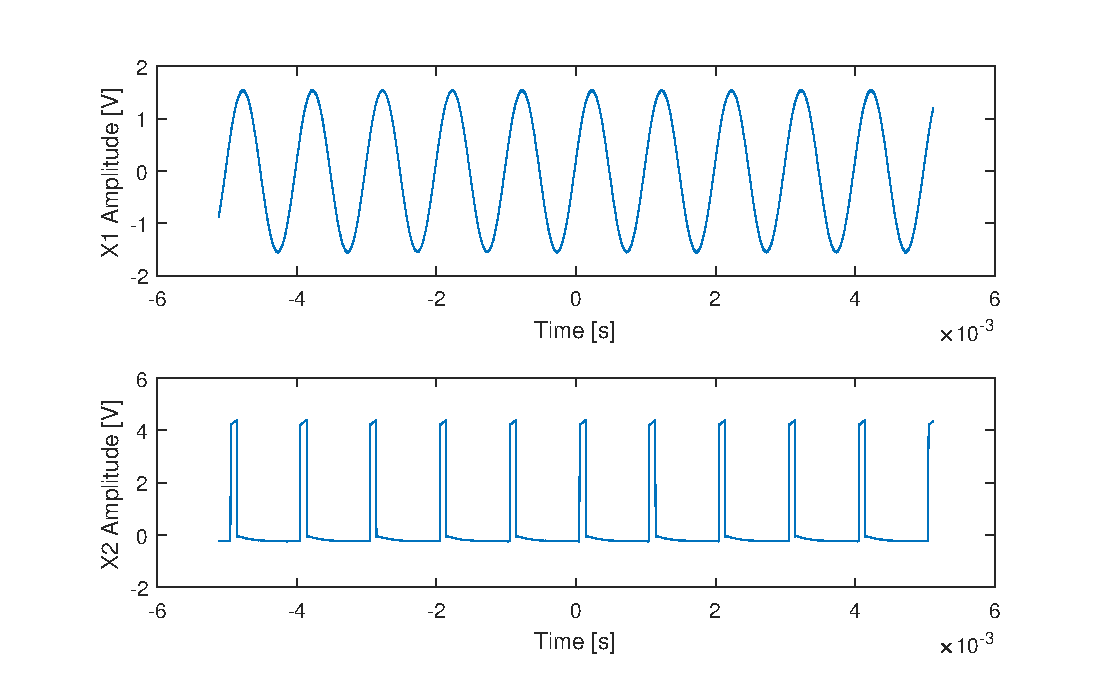
\includegraphics[trim={1cm 0cm 1cm 0cm},clip,width=\textwidth]{img/X1-X2.eps}
    \caption{X1 X2}
    \label{fig:m_x1-x2}
\end{figure}

Here we see that the sinusoidal signal X1 with zero DC component is transformed into a two level signal X2 between 0V and 5V. We also see that it has a constant duty cycle.

\Cref{fig:m_x1-x2-x4-x8} shows the same signals X1 and X2 as in \cref{fig:m_x1-x2} but also shows the output of the interrupter X4 as well as the feedback signal X8. Note that X2 is measured after the optical channel.

\begin{figure}[H]
    \centering
    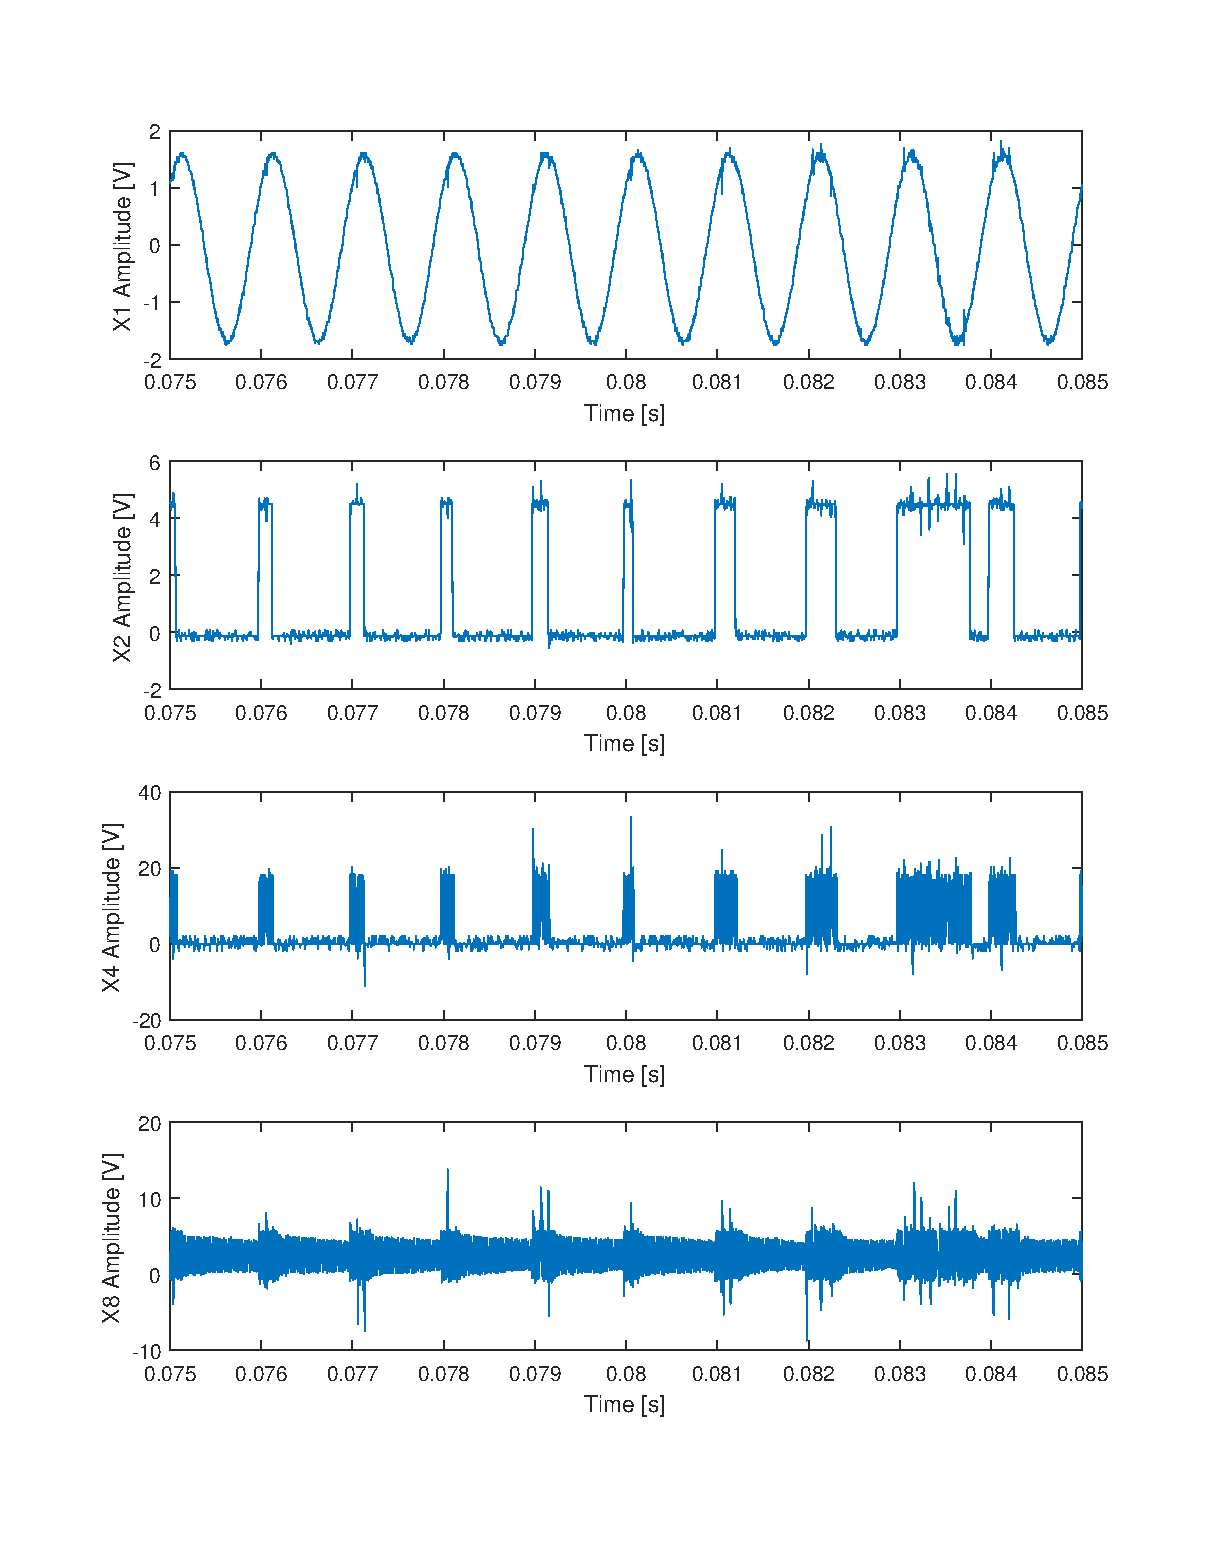
\includegraphics[trim={1cm 0cm 1cm 0cm},clip,width=\textwidth]{img/X1-X2-X4-X8.eps}
    \caption{X1 X2 X4 X8}
    \label{fig:m_x1-x2-x4-x8}
\end{figure}

First it is worth noting that we have more noise in \cref{fig:m_x1-x2-x4-x8} than in \cref{fig:m_x1-x2} because the interrupter, power amplifier, and resonant circuit are connected and turned on. We see that this electromagnetic noise affects how well X2 is generated, and the duty cycle is no longer constant. This is a source of noise on the output acoustic signal. The envelope of X4 follows X2 as expected. The envelope of X8 follows X2 as well as it having a ring down.

\Cref{fig:m_x6} shows the voltage on the output of the power amplifier $U_{X6}$.

\begin{figure}[H]
    \centering
    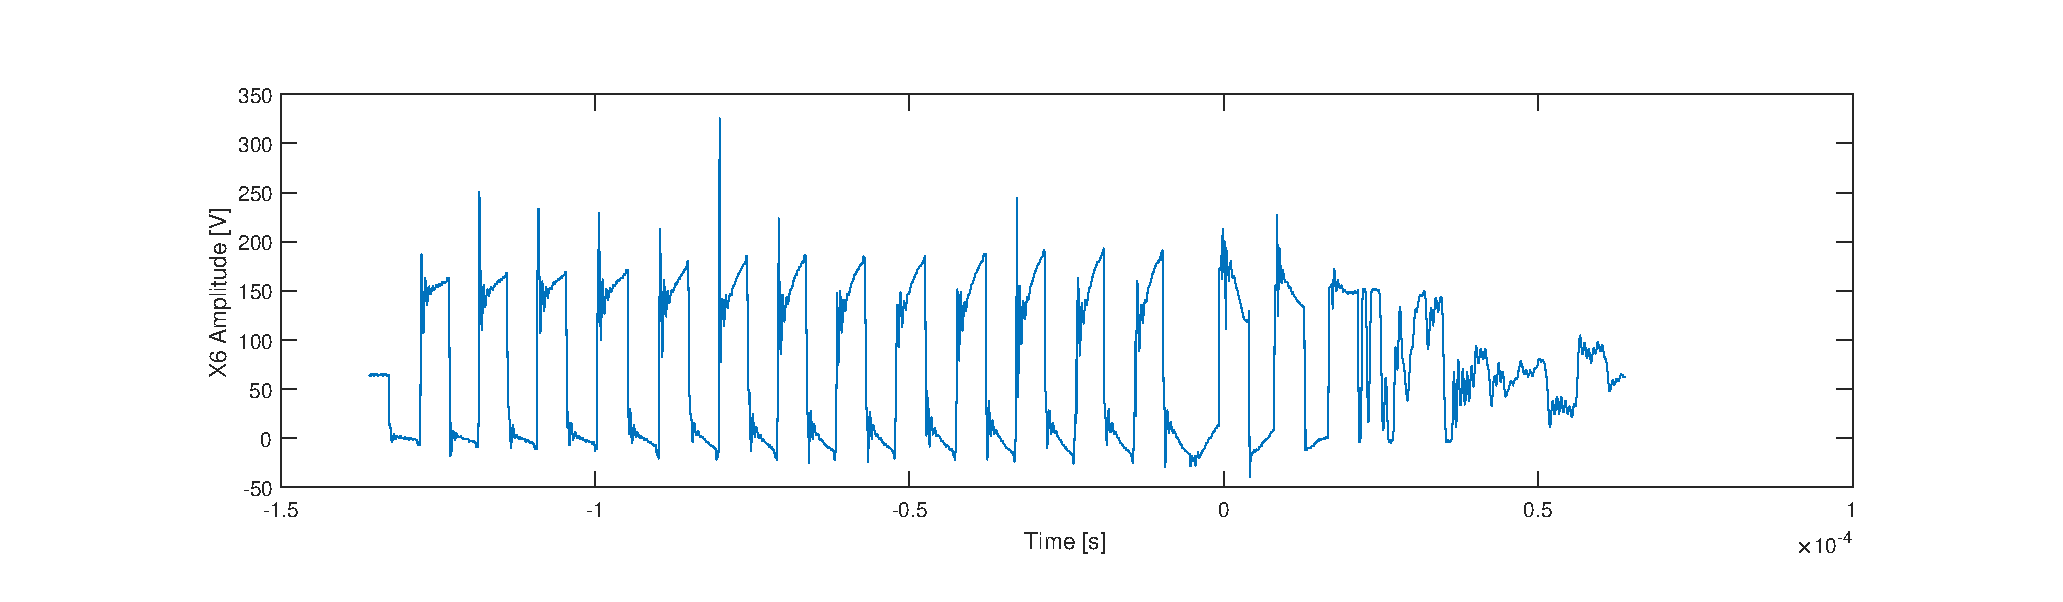
\includegraphics[trim={3.2cm 0cm 3.2cm 0cm},clip,width=\textwidth]{img/X6singlepulse.eps}
    \caption{X6}
    \label{fig:m_x6}
\end{figure}

Here we see a positive square wave with 50\% duty cycle and amplitude from 0V to 160V, and a duration of 13 cycles before being turned off. After this wave train we see the ring down of the voltage on the resonant circuit.

\newpage
\section{Acoustic measurements}

\Cref{fig:period_1k} shows a periodogram of the recorded audio signal with a 1kHz input on X2. The amplitude is the energy of the signal and the x-axis shows the frequency.
\begin{figure}[H]
    \centering
    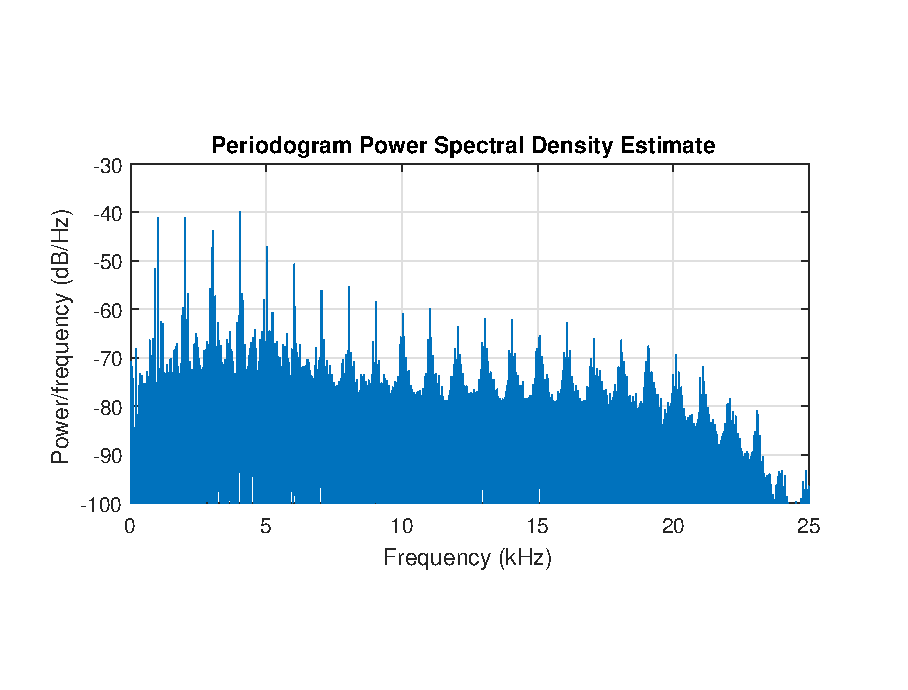
\includegraphics[trim={0cm 1.6cm 0cm 2cm},clip,width=\textwidth]{img/Periodogram_1khz-09.eps}
    \caption{Periodogram of 1kHz recorded tone}
    \label{fig:period_1k}
\end{figure}

Here we see the base frequency 1kHz and harmonics spaced 1kHz apart all the way through the range of human hearing. We see that the lowest three harmonics together with the base frequency are dominant, then the energy of the harmonics start to decrease. This implies the waveform rises sharply and has a short duration, which is consistent with a series of electrical discharges. The amplitudes of the harmonics are shown in \cref{tab:1k_amps}.

\Cref{fig:recorded_1k} shows the waveform of the recorded audio signal with a 1kHz input on X2.

\begin{figure}[H]
    \centering
    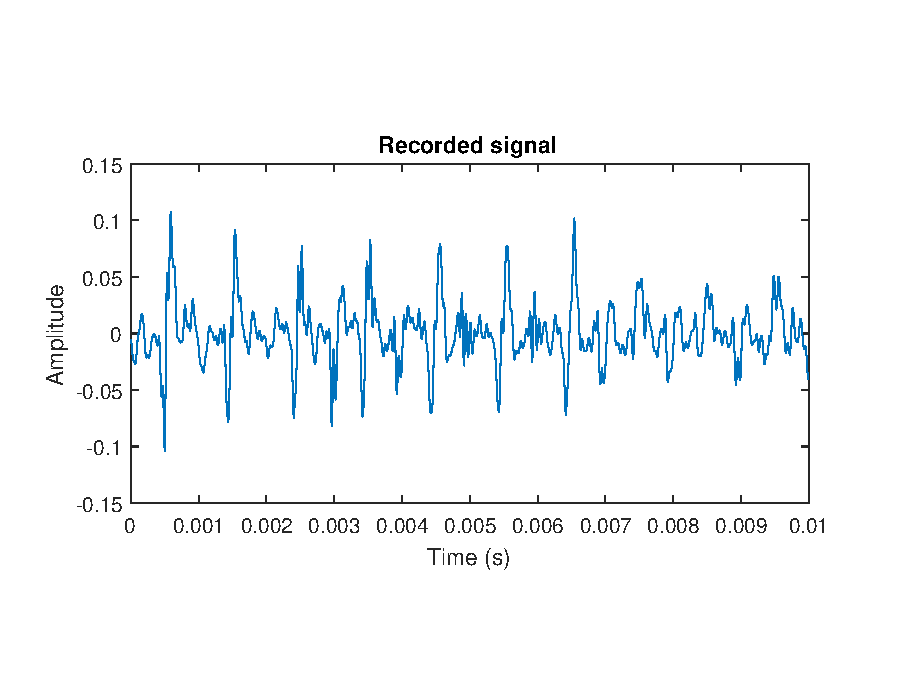
\includegraphics[trim={0cm 1.6cm 0cm 2cm},clip,width=\textwidth]{img/Recorded_1khz-09.eps}
    \caption{Time domain plot of 1kHz recorded tone}
    \label{fig:recorded_1k}
\end{figure}

Here we see a dominant series of pulses with frequency 1kHz, we also see that it has several higher harmonics. Which is consistent with \cref{fig:period_1k}. The signal also appears to be noisy.

%\begin{table}[]
%    \centering
%    \begin{tabular}{c|c|c|c|c|c|c|c|c|c|c|c|c|c|c|c|c|c|c|c|c|c|c}
%        Frequency (Hz)      & 1k  & 2k  & 3k  & 4k  & 5k  & 6k  & 7k  & 8k  & 9k  & 10k & 11k & 12k & 13k & 14k & 15k & 16k & 17k & 18k & 19k & 20k & 21k & 22k \\
%        Amplitude (dB/Hz)   & -41 & -41 & -44 & -40 & -47 & -51 & -55 & -55 & -58 & -60 & -60 & -64 & -62 & -62 & -65 & -62 & -66 & -66 & -67 & -70 & -72 & -80 \\
%    \end{tabular}
%    \caption{Caption}
%    \label{tab:my_label}
%\end{table}

\begin{table}[h]
    \centering
    \begin{tabular}{c|c}
        Frequency (Hz) & Amplitude (dB/Hz) \\
        1k  & -41 \\
        2k  & -41 \\
        3k  & -44 \\
        4k  & -40 \\
        5k  & -47 \\
        6k  & -51 \\
        7k  & -55 \\
        8k  & -55 \\
        9k  & -58 \\
        10k & -60 \\
        11k & -60 \\
        12k & -64 \\
        13k & -62 \\
        14k & -62 \\
        15k & -65 \\
        16k & -62 \\
        17k & -66 \\
        18k & -66 \\
        19k & -67 \\
        20k & -70 \\
        21k & -72 \\
        22k & -80
    \end{tabular}
    \caption{Amplitudes of the harmonics}
    \label{tab:1k_amps}
\end{table}

\Cref{fig:rectones} shows the recorded signal compared to a signal generated in matlab with the amplitudes read from the periodogram of the recorded signal and shown in \cref{tab:1k_amps}.

\begin{figure}[H]
    \centering
    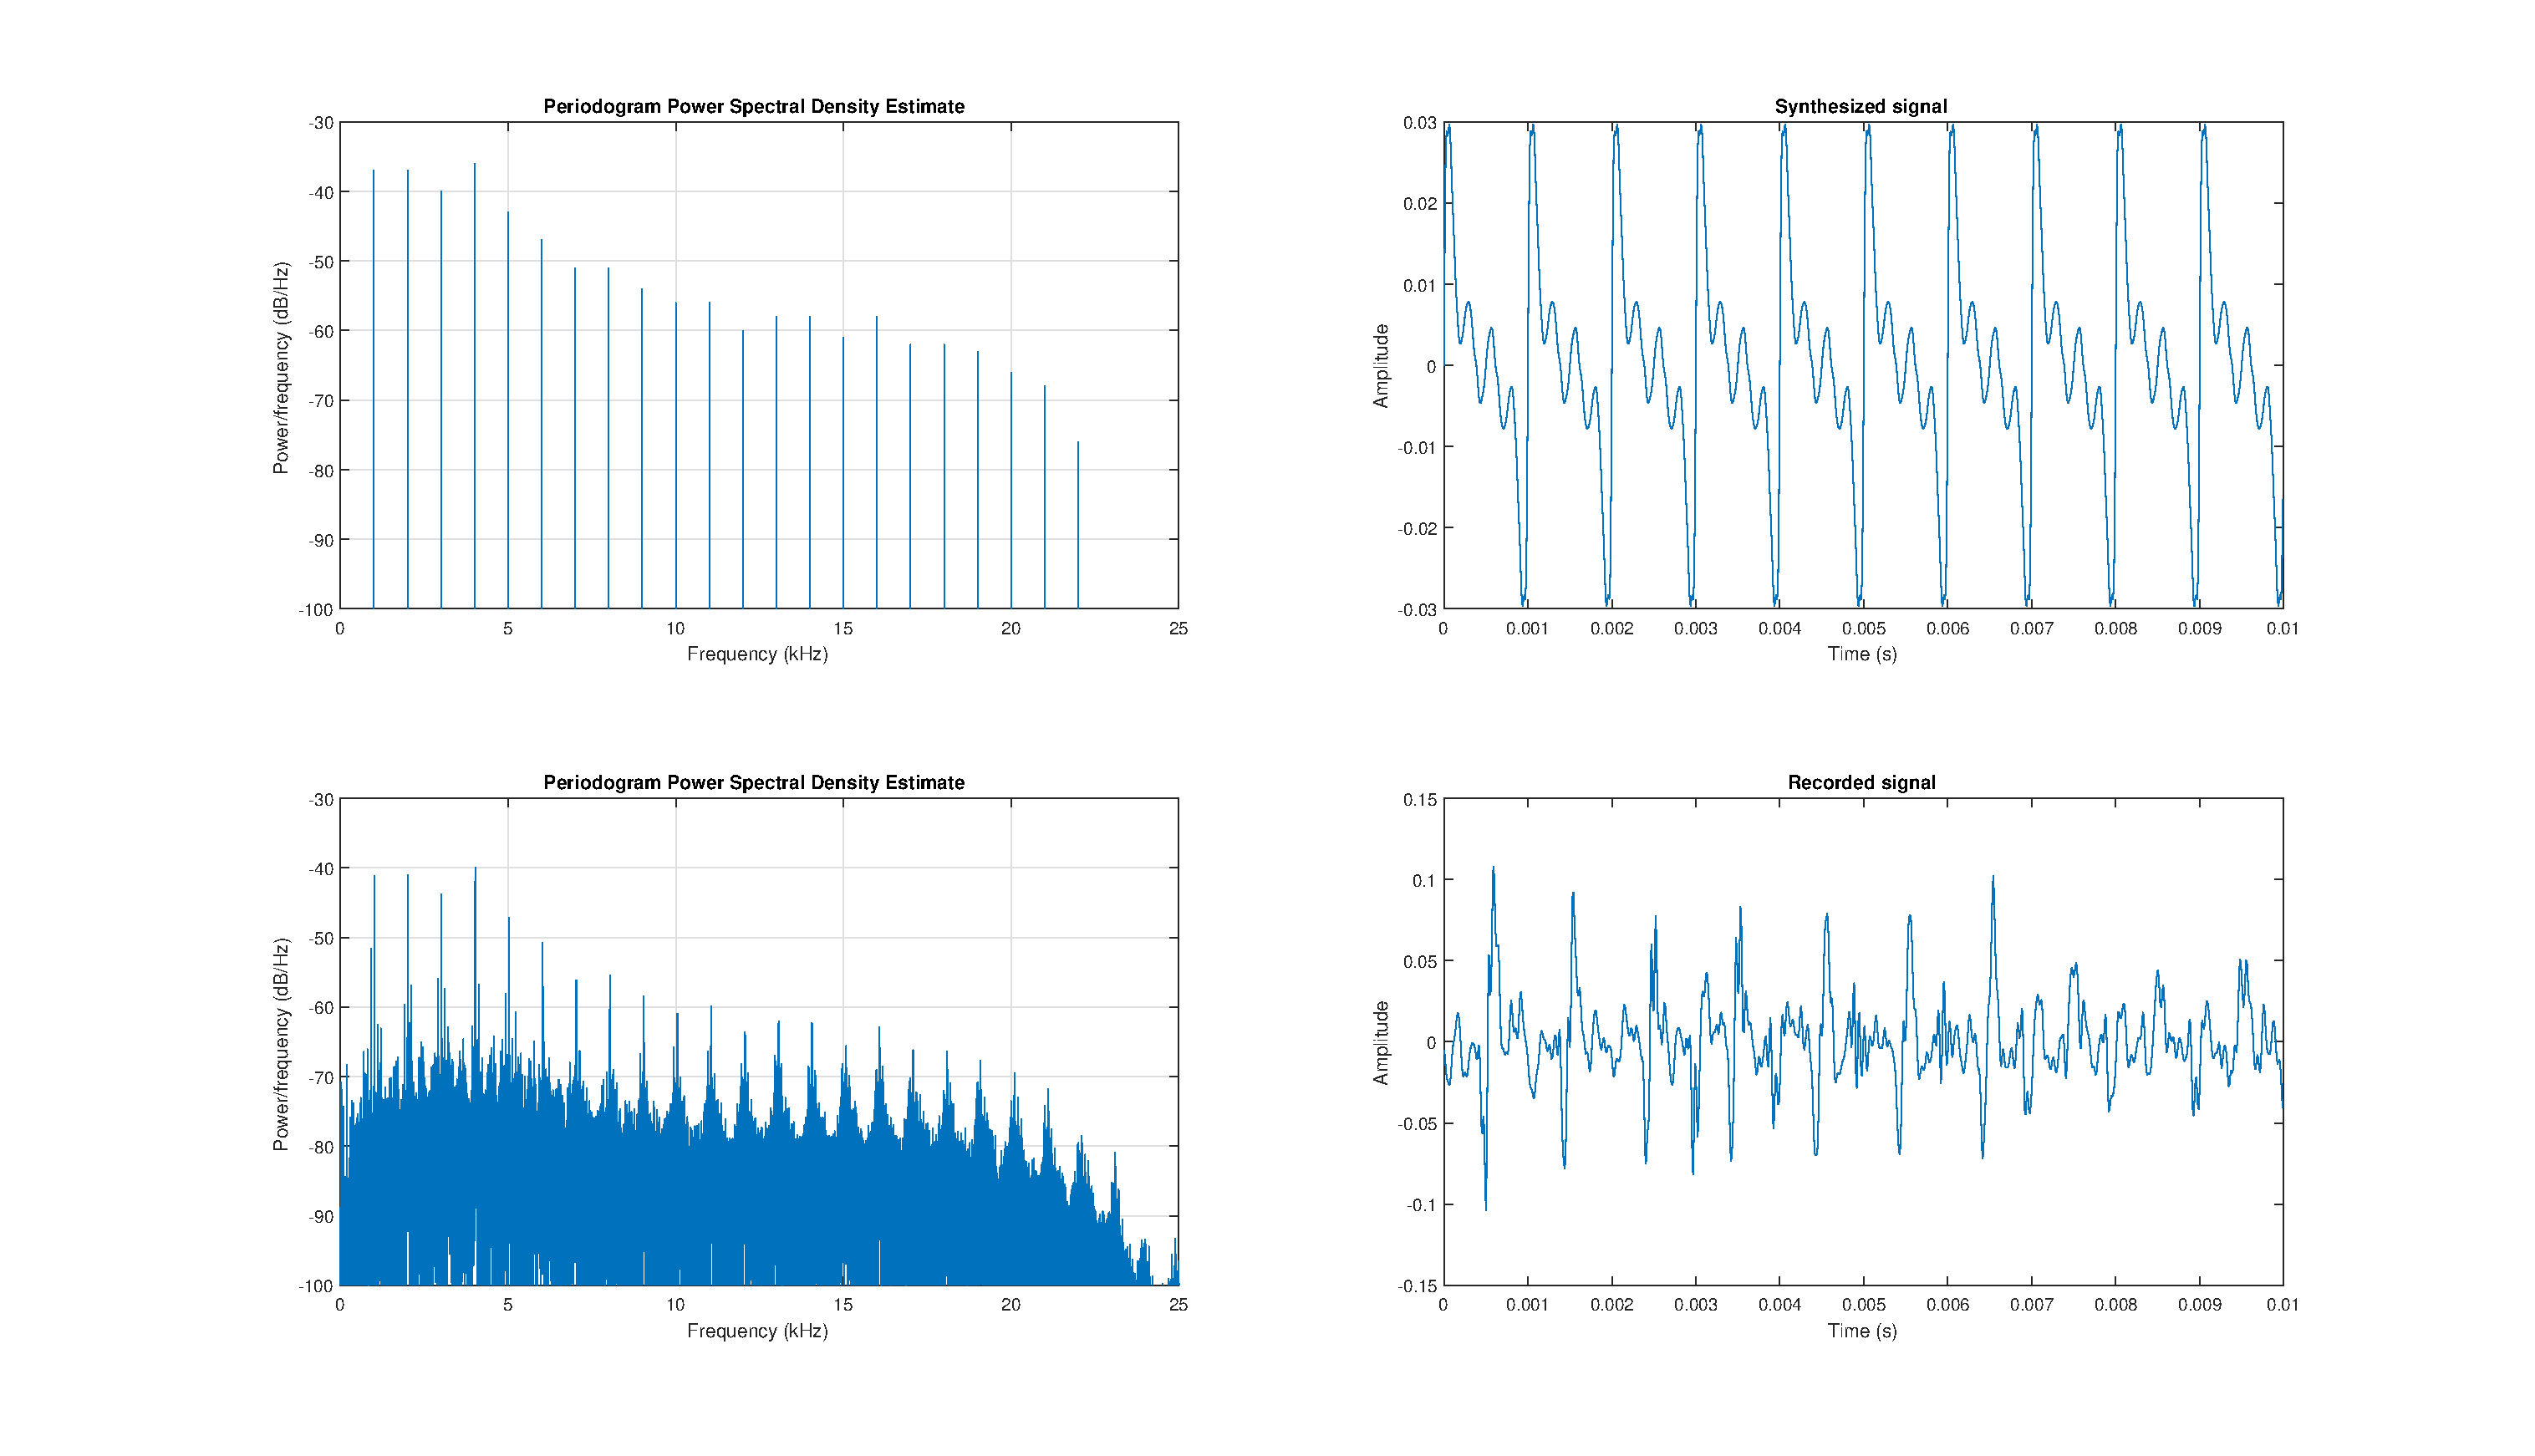
\includegraphics[trim={4cm 1.6cm 4cm 1.6cm},clip,width=\textwidth]{img/tones.eps}
    \caption{Comparison of recorded tone and synthesized tone}
    \label{fig:rectones}
\end{figure}

From this figure we see that the reconstructed signal matches well with the exception of the reconstructed signal not having any frequency components other than the harmonics.